#include "main.typ"
\section{Dạng toán về cực trị hàm trùng phương}

\noindent \textbf{Hàm trùng phương:} \\
Cho hàm số trùng phương $y = ax^4 + bx^2 + c$ ($a \neq 0$) có $ab < 0$. Đồ thị hàm số có 3 điểm cực trị tạo thành tam giác $ABC$ cân tại $A$:
\begin{itemize}
    \item $A(0; c)$ thuộc trục tung.
    \item $B\left(-\sqrt{-\dfrac{b}{2a}}; c - \dfrac{b^2}{4a}\right)$, \quad $C\left(\sqrt{-\dfrac{b}{2a}}; c - \dfrac{b^2}{4a}\right)$.
    \item $BC^2 = -\dfrac{2b}{a}$, \quad $AB^2 = AC^2 = \dfrac{b^4 - 8ab}{16a^2}$.
\end{itemize}
\noindent Đặt : $\widehat{BAC} = \alpha$

\[
\text{Tổng quát: } \boxed{\cot^2 \frac{\alpha}{2} = \frac{-b^3}{8a}}
\]
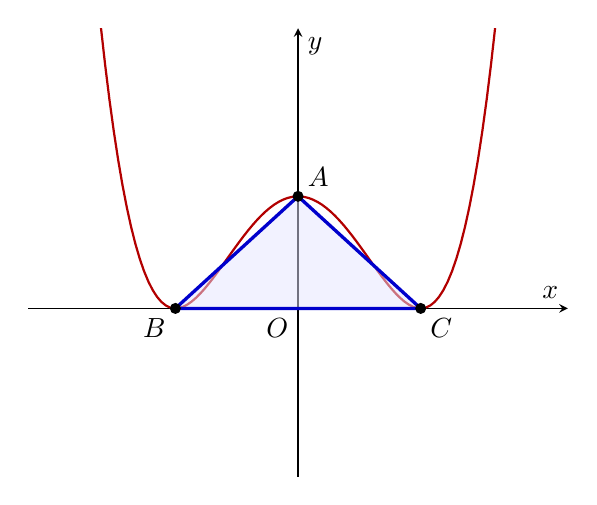
\begin{tikzpicture}
  \begin{axis}[
    axis lines = center,
    xlabel = {$x$},
    ylabel = {$y$},
    xmin = -2.2, xmax = 2.2,
    ymin = -1.5, ymax = 2.5,
    ticks = none,
    enlargelimits = false
  ]
    % Vẽ đồ thị hàm trùng phương y = x^4 - 2x^2 + 1
    \addplot [domain=-1.75:1.75, samples=100, color=red!70!black, thick] {x^4 - 2*x^2 + 1};

    % Tọa độ 3 điểm cực trị: A(0,1), B(-1,0), C(1,0)
    \coordinate (A) at (axis cs:0, 1);
    \coordinate (B) at (axis cs:-1, 0);
    \coordinate (C) at (axis cs:1, 0);

    % Vẽ tam giác ABC
    \draw[line width=1.2pt, blue!80!black, fill=blue!10, fill opacity=0.5] (A) -- (B) -- (C) -- cycle;

    % Chấm các điểm A, B, C
    \fill [black] (A) circle (2pt) node[above right] {$A$};
    \fill [black] (B) circle (2pt) node[below left] {$B$};
    \fill [black] (C) circle (2pt) node[below right] {$C$};
    \node [below left] at (axis cs:0,0) {$O$};
  \end{axis}
\end{tikzpicture}
\vspace{0.5cm}
\subsection{Nhận xét:}
$\Delta ABC$ cân tại $A$, có $A \in Oy$, $AB = AC = \sqrt{\dfrac{b^4 - 8ab}{16a^2}}$, $BC = \sqrt{\dfrac{-2b}{a}}$.

\begin{itemize}
    \item Các điểm cực trị đồ thị hàm số thuộc các trục tọa độ $\Leftrightarrow b^2 = 4ac$.
    \item Điểm $(0; y_0)$ là trọng tâm tam giác $ABC \Leftrightarrow 3y_0 = 3c - \dfrac{b^2}{2a}$.
    \item Điểm $(0; y_0)$ là trực tâm tam giác $ABC \Leftrightarrow y_0 - c = -\dfrac{8a + b^3}{4ab}$.
    \item Điểm $(0; y_0)$ là tâm ngoại tiếp $ABC \Leftrightarrow y_0 - c = \dfrac{8a - b^3}{8ab}$.
\end{itemize}

\noindent Do đó $\cos \angle BAC = \dfrac{b^3 + 8a}{b^3 - 8a}$ và $S_{\Delta ABC} = \sqrt{\dfrac{-b^5}{32a^3}}$.

\begin{itemize}
    \item Tam giác $ABC$ vuông tại $A \Leftrightarrow \cos \angle BAC = 0 \Leftrightarrow b^3 = -8a$.
    \item Tam giác $ABC$ đều $\Leftrightarrow \cos \angle BAC = \dfrac{1}{2} \Leftrightarrow b^3 = -24a$.
    \item Tam giác $ABC$ có một góc $120^\circ \Leftrightarrow \cos \angle BAC = -\dfrac{1}{2} \Leftrightarrow 3b^3 = -8a$.
\end{itemize}
\subsection{Giao điểm với trục 0y}
\noindent Với $ab < 0, ac > 0, b^2 - 4ac > 0$ đồ thị hàm số cắt trục hoành tại 4 điểm phân biệt. \\
Khi đó:

\begin{itemize}
    \item Hoành độ 4 giao điểm lập thành cấp số cộng $\Leftrightarrow 9b^2 = 100ac$.
    \item Cắt trục hoành tại 4 điểm phân biệt, tạo thành 3 đoạn thẳng có độ dài bằng nhau $\Leftrightarrow 9b^2 = 100ac$.
    \item Diện tích hình phẳng giới hạn bởi đồ thị hàm số và trục hoành có phần phía trên $Ox$ và phần phía dưới $Ox$ bằng nhau $\Leftrightarrow 5b^2 = 36ac$.
\end{itemize}
\subsection{MỘT SỐ CÔNG THỨC NHANH}
% ================= CÔNG THỨC 1 =================
\subsubsection{CÔNG THỨC 1: Góc tại đỉnh cực trị $\widehat{BAC} = \alpha$}

\noindent \textbf{Chứng minh:} \\
Áp dụng định lý cosin trong $\triangle ABC$ cân tại $A$:
\[
\cos \alpha = \frac{AB^2 + AC^2 - BC^2}{2 \cdot AB \cdot AC} = 1 - \frac{BC^2}{2AB^2}
\]
Thay $BC^2 = -\dfrac{2b}{a}$ và $AB^2 = \dfrac{b^4 - 8ab}{16a^2}$ vào biểu thức:
\[
\cos \alpha = 1 - \frac{-\dfrac{2b}{a}}{2 \cdot \dfrac{b^4 - 8ab}{16a^2}} = 1 + \frac{16a}{b^3 - 8a} = \frac{b^3 + 8a}{b^3 - 8a}
\]
Mặt khác, sử dụng công thức lượng giác nửa góc:
\[
\tan^2 \frac{\alpha}{2} = \frac{1 - \cos \alpha}{1 + \cos \alpha} = \frac{1 - \dfrac{b^3 + 8a}{b^3 - 8a}}{1 + \dfrac{b^3 + 8a}{b^3 - 8a}} = -\frac{8a}{b^3}
\]

\begin{tcolorbox}[title=CÔNG THỨC GIẢI NHANH 1]
\[
\cos \alpha = \frac{b^3 + 8a}{b^3 - 8a} \quad \text{hoặc} \quad \tan^2 \frac{\alpha}{2} = -\frac{8a}{b^3}
\]
\end{tcolorbox}

\noindent \textbf{Ví dụ minh họa:} \\
\textbf{Bài toán:} Tìm tham số $m$ để đồ thị hàm số $y = x^4 - 2mx^2 + 1$ có 3 điểm cực trị $A, B, C$ sao cho góc $\widehat{BAC} = 120^\circ$.

\noindent \textbf{Lời giải:}
\begin{itemize}
    \item Hàm số có các hệ số: $a = 1$, $b = -2m$.
    \item Điều kiện để hàm số có 3 điểm cực trị: $ab < 0 \iff 1 \cdot (-2m) < 0 \iff m > 0$.
    \item Áp dụng Công thức 1 với $\alpha = 120^\circ \implies \dfrac{\alpha}{2} = 60^\circ$:
    \[
    \tan^2(60^\circ) = -\frac{8a}{b^3} \iff (\sqrt{3})^2 = -\frac{8(1)}{(-2m)^3} \iff 3 = \frac{8}{8m^3} \iff 3 = \frac{1}{m^3}
    \]
    \[
    \iff m^3 = \frac{1}{3} \iff m = \frac{1}{\sqrt[3]{3}} \quad (\text{Thỏa mãn condition } m > 0)
    \]
\end{itemize}

\vspace{0.5cm}

% ================= CÔNG THỨC 2 =================
\subsubsection{CÔNG THỨC 2: Tam giác cực trị $ABC$ vuông cân tại $A$}

\noindent \textbf{Chứng minh:} \\
\textit{Cách 1:} $\triangle ABC$ vuông tại $A \iff \widehat{BAC} = 90^\circ \iff \cos \alpha = 0$. \\
Thay vào Công thức 1 ta có:
\[
\cos \alpha = 0 \iff \frac{b^3 + 8a}{b^3 - 8a} = 0 \iff b^3 + 8a = 0
\]

\noindent \textit{Cách 2 (Định lý Pitago):} $\triangle ABC$ vuông cân $\iff BC^2 = AB^2 + AC^2 = 2AB^2$
\[
\iff -\frac{2b}{a} = 2\left(\frac{b^4}{16a^2} - \frac{b}{2a}\right) \iff \frac{b^4}{16a^2} + \frac{b}{2a} = 0 \iff b^3 + 8a = 0
\]

\begin{tcolorbox}[title=CÔNG THỨC GIẢI NHANH 2]
\[
b^3 + 8a = 0
\]
\end{tcolorbox}

\noindent \textbf{Ví dụ minh họa:} \\
\textbf{Bài toán:} Tìm tham số $m$ để đồ thị hàm số $y = x^4 - 2mx^2 + 1$ có 3 điểm cực trị $A, B, C$ tạo thành một tam giác vuông cân tại $A$.

\noindent \textbf{Lời giải:}
\begin{itemize}
    \item Hàm số có các hệ số: $a = 1$, $b = -2m$.
    \item Điều kiện để hàm số có 3 điểm cực trị: $ab < 0 \iff 1 \cdot (-2m) < 0 \iff m > 0$.
    \item Áp dụng Công thức 2: $b^3 + 8a = 0$:
    \[
    (-2m)^3 + 8(1) = 0 \iff -8m^3 + 8 = 0 \iff m^3 = 1 \iff m = 1 \quad (\text{Thỏa mãn condition } m > 0)
    \]
\end{itemize}
% ================= CÔNG THỨC 3 =================
\subsubsection{CÔNG THỨC 3: Tam giác cực trị $ABC$ đều}

\noindent \textbf{Chứng minh:} \\
Vì $\triangle ABC$ luôn cân tại $A$, để $\triangle ABC$ đều thì $\widehat{BAC} = 60^\circ \iff \cos \alpha = \cos 60^\circ = \dfrac{1}{2}$. \\
Thế vào công thức góc:
\[
\cos \alpha = \frac{1}{2} \iff \frac{b^3 + 8a}{b^3 - 8a} = \frac{1}{2} \iff 2(b^3 + 8a) = b^3 - 8a \iff b^3 + 24a = 0
\]
\textit{Hoặc dùng độ dài cạnh:} $\triangle ABC$ đều $\iff BC^2 = AB^2$:
\[
-\frac{2b}{a} = \frac{b^4 - 8ab}{16a^2} \iff \frac{b^4}{16a^2} + \frac{3b}{2a} = 0 \iff b^3 + 24a = 0 \quad (\text{do } b \neq 0)
\]

\begin{tcolorbox}[title=CÔNG THỨC GIẢI NHANH 3]
\[
b^3 + 24a = 0
\]
\end{tcolorbox}

\noindent \textbf{Ví dụ minh họa:} \\
\textbf{Bài toán:} Tìm tham số $m$ để đồ thị hàm số $y = x^4 - 2mx^2 + 2$ có 3 điểm cực trị tạo thành một tam giác đều.

\noindent \textbf{Lời giải:}
\begin{itemize}
    \item Hệ số: $a = 1$, $b = -2m$. Điều kiện có 3 điểm cực trị: $ab < 0 \iff m > 0$.
    \item Áp dụng Công thức 3: $b^3 + 24a = 0$:
    \[
    (-2m)^3 + 24(1) = 0 \iff -8m^3 + 24 = 0 \iff m^3 = 3 \iff m = \sqrt[3]{3} \quad (\text{Thỏa mãn } m > 0)
    \]
\end{itemize}


\vspace{0.5cm}

% ================= CÔNG THỨC 4 =================
\subsubsection{CÔNG THỨC 4: Diện tích tam giác cực trị $S_{\triangle ABC}$}

\noindent \textbf{Chứng minh:} \\
Gọi $I$ là trung điểm của $BC$. Do $\triangle ABC$ cân tại $A$ nên $AI \perp BC$. \\
Tọa độ $I\left(0; c - \dfrac{b^2}{4a}\right) \implies AI = \left|y_A - y_I\right| = \left|c - \left(c - \dfrac{b^2}{4a}\right)\right| = \dfrac{b^2}{4|a|} = -\dfrac{b^2}{4a}$. \\
Độ dài $BC = 2\sqrt{-\dfrac{b}{2a}}$. \\
Diện tích tam giác $ABC$:
\[
S_{\triangle ABC} = \frac{1}{2} BC \cdot AI = \frac{1}{2} \cdot 2\sqrt{-\frac{b}{2a}} \cdot \left(-\frac{b^2}{4a}\right) = |a| \left(\sqrt{-\frac{b}{2a}}\right)^5
\]

\begin{tcolorbox}[title=CÔNG THỨC GIẢI NHANH 4]
\[
S_{\triangle ABC} = |a| \left(\sqrt{-\frac{b}{2a}}\right)^5 \quad \text{hoặc} \quad 32 a^3 S^2 + b^5 = 0
\]
\end{tcolorbox}

\noindent \textbf{Ví dụ minh họa:} \\
\textbf{Bài toán:} Tìm $m$ để đồ thị hàm số $y = x^4 - 2mx^2$ có 3 điểm cực trị $A, B, C$ sao cho $S_{\triangle ABC} = 4$.

\noindent \textbf{Lời giải:}
\begin{itemize}
    \item Hệ số: $a = 1$, $b = -2m$. Điều kiện có 3 điểm cực trị: $m > 0$.
    \item Áp dụng Công thức 4 với $S = 4$:
    \[
    32 a^3 S^2 + b^5 = 0 \iff 32(1)^3(4)^2 + (-2m)^5 = 0 \iff 512 - 32m^5 = 0 \iff m^5 = 16 \iff m = \sqrt[5]{16}
    \]
\end{itemize}

\vspace{0.5cm}

% ================= CÔNG THỨC 5 =================
\subsubsection{CÔNG THỨC 5: Bán kính đường tròn ngoại tiếp $R_{\triangle ABC}$}

\noindent \textbf{Chứng minh:} \\
Áp dụng công thức tính diện tích tam giác $S = \dfrac{AB \cdot AC \cdot BC}{4R} = \dfrac{AB^2 \cdot BC}{4R} \implies R = \dfrac{AB^2 \cdot BC}{4S}$. \\
Thay $AB^2 = \dfrac{b^4 - 8ab}{16a^2}$, $BC = 2\sqrt{-\dfrac{b}{2a}}$ và $S = \dfrac{b^2}{4|a|}\sqrt{-\dfrac{b}{2a}}$ vào:
\[
R = \frac{\dfrac{b^4 - 8ab}{16a^2} \cdot 2\sqrt{-\dfrac{b}{2a}}}{4 \cdot \dfrac{b^2}{4|a|}\sqrt{-\dfrac{b}{2a}}} = \frac{b^4 - 8ab}{8a^2} \cdot \frac{|a|}{b^2} = \frac{b(b^3 - 8a)}{8a^2} \cdot \frac{|a|}{b^2} = \frac{b^3 - 8a}{8|a|b}
\]

\begin{tcolorbox}[title=CÔNG THỨC GIẢI NHANH 5]
\[
R = \frac{b^3 - 8a}{8|a|b}
\]
\end{tcolorbox}

\noindent \textbf{Ví dụ minh họa:} \\
\textbf{Bài toán:} Tìm $m$ để đồ thị hàm số $y = x^4 - 2mx^2 + 1$ có 3 điểm cực trị $A, B, C$ sao cho bán kính đường tròn ngoại tiếp $\triangle ABC$ bằng $1$.

\noindent \textbf{Lời giải:}
\begin{itemize}
    \item Hệ số: $a = 1$, $b = -2m$. Điều kiện có 3 điểm cực trị: $m > 0$.
    \item Áp dụng Công thức 5 với $R = 1$:
    \[
    1 = \frac{(-2m)^3 - 8(1)}{8|1|(-2m)} \iff 1 = \frac{-8m^3 - 8}{-16m} \iff 16m = 8m^3 + 8 \iff m^3 - 2m + 1 = 0
    \]
    \[
    \iff (m - 1)(m^2 + m - 1) = 0 \iff \left[ \begin{array}{l} m = 1 \\ m = \dfrac{-1 + \sqrt{5}}{2} \quad (\text{do } m > 0) \end{array} \right.
    \]
\end{itemize}
% ================= CÔNG THỨC 6 =================
\subsubsection{CÔNG THỨC 6: Bán kính đường tròn nội tiếp $r_{\triangle ABC}$}

\noindent \textbf{Chứng minh:} \\
Bán kính đường tròn nội tiếp tam giác được tính theo công thức $r = \dfrac{S}{p}$, trong đó $S$ là diện tích và $p$ là nửa chu vi của $\triangle ABC$:
\[
p = \frac{BC + 2AB}{2} = \sqrt{-\frac{b}{2a}} + \sqrt{\frac{b^4 - 8ab}{16a^2}} = \sqrt{-\frac{b}{2a}} + \frac{\sqrt{b^4 - 8ab}}{4|a|}
\]
Thay $S = \dfrac{b^2}{4|a|}\sqrt{-\dfrac{b}{2a}}$ vào công thức $r = \dfrac{S}{p}$:
\[
r = \frac{\dfrac{b^2}{4|a|}\sqrt{-\dfrac{b}{2a}}}{\sqrt{-\dfrac{b}{2a}} + \dfrac{\sqrt{b^4 - 8ab}}{4|a|}} = \frac{b^2}{4|a| + \sqrt{16a^2 - 2ab^3}}
\]

\begin{tcolorbox}[title=CÔNG THỨC GIẢI NHANH 6]
\[
r = \frac{b^2}{4|a| + \sqrt{16a^2 - 2ab^3}}
\]
\end{tcolorbox}

\noindent \textbf{Ví dụ minh họa:} \\
\textbf{Bài toán:} Cho hàm số $y = x^4 - 2x^2 + 1$. Tính bán kính đường tròn nội tiếp $r$ của tam giác tạo bởi 3 điểm cực trị.

\noindent \textbf{Lời giải:}
\begin{itemize}
    \item Các hệ số: $a = 1$, $b = -2$, $c = 1$.
    \item Do $ab = -2 < 0$, hàm số có 3 điểm cực trị.
    \item Áp dụng Công thức 6:
    \[
    r = \frac{(-2)^2}{4|1| + \sqrt{16(1)^2 - 2(1)(-2)^3}} = \frac{4}{4 + \sqrt{16 + 16}} = \frac{4}{4 + 4\sqrt{2}} = \sqrt{2} - 1
    \]
\end{itemize}
\vspace{0.5cm}

% ================= CÔNG THỨC 7 =================
\subsubsection{CÔNG THỨC 7: $\triangle ABC$ có trọng tâm là gốc tọa độ $O(0;0)$}

\noindent \textbf{Chứng minh:} \\
Tọa độ 3 điểm cực trị là $A(0; c)$, $B\left(-\sqrt{-\frac{b}{2a}}; c - \frac{b^2}{4a}\right)$, $C\left(\sqrt{-\frac{b}{2a}}; c - \frac{b^2}{4a}\right)$. \\
Toạ độ trọng tâm $G$ của $\triangle ABC$ thỏa mãn $y_G = \dfrac{y_A + y_B + y_C}{3} = \dfrac{c + 2\left(c - \dfrac{b^2}{4a}\right)}{3} = c - \dfrac{b^2}{6a}$. \\
Tam giác $ABC$ có trọng tâm $G \equiv O(0;0) \iff y_G = 0$:
\[
c - \frac{b^2}{6a} = 0 \iff 6ac - b^2 = 0 \iff b^2 - 6ac = 0
\]

\begin{tcolorbox}[title=CÔNG THỨC GIẢI NHANH 7]
\[
b^2 - 6ac = 0
\]
\end{tcolorbox}

\noindent \textbf{Ví dụ minh họa:} \\
\textbf{Bài toán:} Tìm $m$ để đồ thị hàm số $y = x^4 - 2mx^2 + m - 1$ có 3 điểm cực trị nhận gốc tọa độ $O$ làm trọng tâm.

\noindent \textbf{Lời giải:}
\begin{itemize}
    \item Hệ số: $a = 1$, $b = -2m$, $c = m - 1$. Điều kiện có 3 cực trị: $m > 0$.
    \item Áp dụng Công thức 7: $b^2 - 6ac = 0$:
    \[
    (-2m)^2 - 6(1)(m - 1) = 0 \iff 4m^2 - 6m + 6 = 0 \quad (\text{Phương trình vô nghiệm})
    \]
    Vậy không tồn tại giá trị $m$ thỏa mãn.
\end{itemize}

\vspace{0.5cm}

% ================= CÔNG THỨC 8 =================
\subsubsection{CÔNG THỨC 8: $\triangle ABC$ có trực tâm là gốc tọa độ $O(0;0)$}

\noindent \textbf{Chứng minh:} \\
Tọa độ $A(0; c)$, $C\left(\sqrt{-\frac{b}{2a}}; c - \frac{b^2}{4a}\right)$, $B\left(-\sqrt{-\frac{b}{2a}}; c - \frac{b^2}{4a}\right) \implies \vec{OB} = \left(-\sqrt{-\frac{b}{2a}}; c - \frac{b^2}{4a}\right)$, $\vec{AC} = \left(\sqrt{-\frac{b}{2a}}; -\frac{b^2}{4a}\right)$. \\
Gốc $O$ là trực tâm $\triangle ABC \iff \vec{OB} \cdot \vec{AC} = 0$:
\[
\left(-\sqrt{-\frac{b}{2a}}\right)\left(\sqrt{-\frac{b}{2a}}\right) + \left(c - \frac{b^2}{4a}\right)\left(-\frac{b^2}{4a}\right) = 0
\]
\[
\iff \frac{b}{2a} - \frac{b^2 c}{4a} + \frac{b^4}{16a^2} = 0 \iff \frac{b}{16a^2} \left(8a - 4ac + b^3\right) = 0 \iff b^3 + 8a - 4ac = 0
\]

\begin{tcolorbox}[title=CÔNG THỨC GIẢI NHANH 8]
\[
b^3 + 8a - 4ac = 0
\]
\end{tcolorbox}

\noindent \textbf{Ví dụ minh họa:} \\
\textbf{Bài toán:} Tìm $m$ để đồ thị hàm số $y = x^4 - 2mx^2 + \dfrac{3}{2}$ có 3 điểm cực trị nhận $O(0;0)$ làm trực tâm.

\noindent \textbf{Lời giải:}
\begin{itemize}
    \item Hệ số: $a = 1$, $b = -2m$, $c = \dfrac{3}{2}$. Điều kiện có 3 cực trị: $m > 0$.
    \item Áp dụng Công thức 8: $b^3 + 8a - 4ac = 0$:
    \[
    (-2m)^3 + 8(1) - 4(1)\left(\frac{3}{2}\right) = 0 \iff -8m^3 + 8 - 6 = 0 \iff 8m^3 = 2 \iff m^3 = \frac{1}{4} \iff m = \frac{1}{\sqrt[3]{4}}
    \]
\end{itemize}


\vspace{0.5cm}

% ================= CÔNG THỨC 9 =================
\subsubsection{CÔNG THỨC 9: Phương trình đường tròn ngoại tiếp $\triangle ABC$}

\noindent \textbf{Chứng minh:} \\
Đường tròn đi qua $A(0; c)$ và hai điểm cực trị $B, C$ đối xứng qua $Oy$ có phương trình dạng:
\[
x^2 + y^2 - 2m y + n = 0
\]
Thế tọa độ các điểm $A, B, C$ và rút gọn theo biến biểu thức $\Delta = b^2 - 4ac$, ta thu được dạng thu gọn chính xác:
\begin{tcolorbox}[title=CÔNG THỨC GIẢI NHANH 9]
\[
x^2 + y^2 - \left( \frac{2}{b} - \frac{\Delta}{4a} + c \right)y + c\left( \frac{2}{b} - \frac{\Delta}{4a} \right) = 0
\]
\end{tcolorbox}

\noindent \textbf{Ví dụ minh họa:} \\
\textbf{Bài toán:} Viết phương trình đường tròn đi qua 3 điểm cực trị của đồ thị hàm số $y = x^4 - 2x^2 + 1$.

\noindent \textbf{Lời giải:}
\begin{itemize}
    \item Hệ số: $a = 1$, $b = -2$, $c = 1$. Tính $\Delta = b^2 - 4ac = (-2)^2 - 4(1)(1) = 0$.
    \item Biểu thức: $\dfrac{2}{b} - \dfrac{\Delta}{4a} = \dfrac{2}{-2} - 0 = -1$.
    \item Áp dụng Công thức 9:
    \[
    x^2 + y^2 - (-1 + 1)y + 1(-1) = 0 \iff x^2 + y^2 - 1 = 0
    \]
\end{itemize}


\vspace{0.5cm}

% ================= CÔNG THỨC 10 =================
\subsubsection{CÔNG THỨC 10: Phương trình Parabol đi qua 3 điểm cực trị}

\noindent \textbf{Chứng minh:} \\
Đạo hàm $y' = 4ax^3 + 2bx = 2x(2ax^2 + b)$. \\
Thực hiện phép chia đa thức $y$ cho $y'$ thu được phần dư bậc 2:
\[
r(x) = -\frac{1}{2}bx^2 + c
\]
Do các điểm cực trị thỏa mãn $y' = 0$ nên tung độ tương ứng sẽ nằm trên đường dư $y = r(x)$.

\begin{tcolorbox}[title=CÔNG THỨC GIẢI NHANH 10]
\[
y = -\frac{1}{2}bx^2 + c
\]
\end{tcolorbox}

\noindent \textbf{Ví dụ minh họa:} \\
\textbf{Bài toán:} Viết phương trình Parabol đi qua 3 điểm cực trị của hàm số $y = x^4 - 4x^2 + 3$.

\noindent \textbf{Lời giải:}
\begin{itemize}
    \item Hệ số: $a = 1$, $b = -4$, $c = 3$.
    \item Áp dụng Công thức 10:
    \[
    y = -\frac{1}{2}(-4)x^2 + 3 \iff y = 2x^2 + 3
    \]
\end{itemize}
\vfill
